\documentclass{standalone}
\usepackage{tikz}
\usetikzlibrary{calc, shapes}

\begin{document}
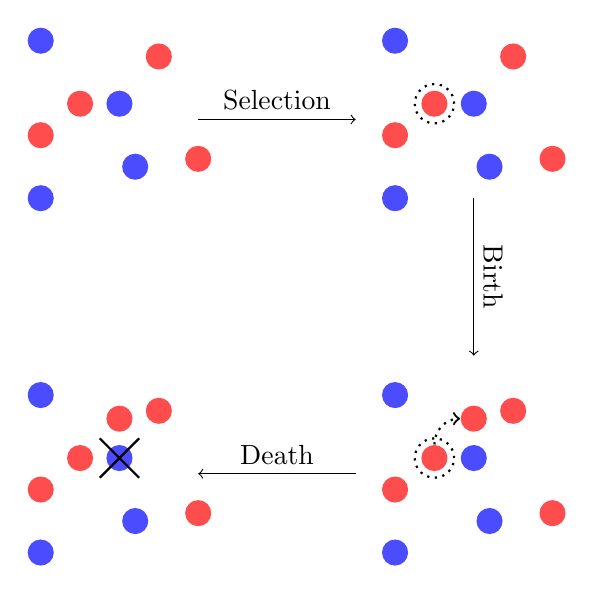
\begin{tikzpicture}
	\node (A1) at (-1, -1) [circle, fill=blue!70] {};
	\node (A2) at (-1, 1) [circle, fill=blue!70] {};
	\node (A3) at (0, .2) [circle, fill=blue!70] {};
	\node (A4) at (.2, -.6) [circle, fill=blue!70] {};
	\node (B1) at (-1, -.2) [circle, fill=red!70] {};
	\node (B2) at (1, -.5) [circle, fill=red!70] {};
	\node (B3) at (.5, .8) [circle, fill=red!70] {};
	\node (B4) at (-.5, .2) [circle, fill=red!70] {};

	\draw [->] (1, 0) -- (3, 0) node [above, pos=0.5] {Selection};

	\node (A1) at ($(A1) + (4.5, 0)$) [circle, fill=blue!70] {};
	\node (A2) at ($(A2) + (4.5, 0)$) [circle, fill=blue!70] {};
	\node (A3) at ($(A3) + (4.5, 0)$) [circle, fill=blue!70] {};
	\node (A4) at ($(A4) + (4.5, 0)$) [circle, fill=blue!70] {};
	\node (B1) at ($(B1) + (4.5, 0)$) [circle, fill=red!70] {};
	\node (B2) at ($(B2) + (4.5, 0)$) [circle, fill=red!70] {};
	\node (B3) at ($(B3) + (4.5, 0)$) [circle, fill=red!70] {};
	\node (B4) at ($(B4) + (4.5, 0)$) [circle, fill=red!70] {};

	\draw [dotted, thick] (B4) circle (.25cm);

	\draw [->] (4.5, -1) -- (4.5, -3) node [above, pos=0.5, rotate=-90] {Birth};

	\node (A1) at ($(A1) + (0, -4.5)$) [circle, fill=blue!70] {};
	\node (A2) at ($(A2) + (0, -4.5)$) [circle, fill=blue!70] {};
	\node (A3) at ($(A3) + (0, -4.5)$) [circle, fill=blue!70] {};
	\node (A4) at ($(A4) + (0, -4.5)$) [circle, fill=blue!70] {};
	\node (B1) at ($(B1) + (0, -4.5)$) [circle, fill=red!70] {};
	\node (B2) at ($(B2) + (0, -4.5)$) [circle, fill=red!70] {};
	\node (B3) at ($(B3) + (0, -4.5)$) [circle, fill=red!70] {};
	\node (B4) at ($(B4) + (0, -4.5)$) [circle, fill=red!70] {};

	\draw [dotted, thick] (B4) circle (.25cm);
	\node (B5) at ($(B4) + (0.5, 0.5)$) [circle, fill=red!70] {};
	\draw [->, dotted, thick] (B4) [out=90, in=180] to (B5);

	\draw [->] (3, -4.5) -- (1, -4.5) node [above, pos=0.5] {Death};

	\node (A1) at ($(A1) + (-4.5, 0)$) [circle, fill=blue!70] {};
	\node (A2) at ($(A2) + (-4.5, 0)$) [circle, fill=blue!70] {};
	\node (A3) at ($(A3) + (-4.5, 0)$) [circle, fill=blue!70] {};
	\node (A4) at ($(A4) + (-4.5, 0)$) [circle, fill=blue!70] {};
	\node (B1) at ($(B1) + (-4.5, 0)$) [circle, fill=red!70] {};
	\node (B2) at ($(B2) + (-4.5, 0)$) [circle, fill=red!70] {};
	\node (B3) at ($(B3) + (-4.5, 0)$) [circle, fill=red!70] {};
	\node (B4) at ($(B4) + (-4.5, 0)$) [circle, fill=red!70] {};
	\node (B5) at ($(B5) + (-4.5, 0)$) [circle, fill=red!70] {};

	\draw [thick] ($(A3) + (-.25, -.25)$) -- ($(A3) + (.25, .25)$);
	\draw [thick] ($(A3) + (.25, -.25)$) -- ($(A3) + (-.25, .25)$);
\end{tikzpicture}
\end{document}
